\chapter{Umsetzung} \label{sec:Umsetzung}

\section{Architektur}
Auf Basis der Grundlagen und Analyse wird die Architektur des Systems erstellt.
In der Architektur werden alle wichtigen Entscheidungen, welche für die
Entwicklung des Systems relevant und von technischer Natur sind, berücksichtigt. Die Architektur dient als Grundlage für die darauffolgende Umsetzung.

\section{Raspberry Pi} HAUPTAUGENMERK AUF BEREITSTELLUNG DER DATEN UND ANZEIGE!!!
Die zentral Einheit um Sensoren in unsere Anwendung zu integrieren bildet der Raspberry Pi. Dabei spielen dessen externe Schnittstellen eine wesentliche Rolle. Allerdings liegt der Fokus dieser Arbeit auf der Datenbereitstellung über einen Webserver und dem Verarbeiten, sowie Anzeigen in der App, weshalb auf bereits bestehende Lösungen zurückgegriffen wird.
\\\\Das \acf{CSI} stellt eine Möglichkeit dar, eine eigens für den Raspberry Pi entworfene Kamera anzuschließen. Das Kameramodul kann dann über entsprechende Befehle über die Kommandozeile des Raspberry gesteuert werden. Aus den Anforderung F-?? geht hervor, dass Bilder bei erkannter Bewegung gespeichert und einen Livestream umgesetzt werden sollen.\\Die Anzeige eines Live-Bildes könnte über eine sekündliche Aufnahme, die über eine Service unter einer Internetadresse verfügbar gemacht wird, umgesetzt werden. Ob innerhalb eines Bildes Bewegung erkannt wurde, könnte durch eine Vergleich eines Referenzbildes und dem aktuellen Bild ermittelt werden.\\Allerdings bietet diese Funktionalitäten bereits das Open-Source Programm \enquote{Motion} an. Es ist in der Lage Bewegung zu erkenne, Live-Bilder anzuzeigen, sowie das Abspeichern von Events bei erkannten Bewegungen\cite{motion:Motion}\\
Motion wird 
\\Motion wurde so konfiguriert, dass der Livestream über die \ac{IP}-Adresse des Raspberry Pis und dem Port 8081 erreichbar ist. Bewegung wird erkannt, wenn sich drei aufeinanderfolgenden Bildern um 15000 Pixel zum Referenzbild unterscheiden. Dabei ist eine Auflösung von 640x480 Pixel gewählt. Wenn für sieben Sekunden keine Bewegung mehr wahrgenommen wird, ist das Event beendet. Für dieses Event wird in der Tabelle Security (siehe \autoref{db:DB}) ein Datenbankeintrag erstellt. Außerdem wird ein Video in einem definierten Verzeichnis abgespeichert, das die ganze Sequenz der Bewegungserkennung enthält. Nachdem das Video erstellt wurde wir außerdem noch ein Bild abgespeichert, das durch die Software analysiert wurde und später dem Anwender der App dargestellt wird.
\\\\
Die Sensoren für Luftfeuchtigkeits- bzw. Temperaturmessung, den Magnetkontakt, sowie den Luftqualitätssensor werden über die Pins des \ac{GPIO} angeschlossen. Im Gegensatz zu MQ-135 Sensor liefern der DHT22 Sensor, und der Magnetsensor digitale Werte zurück. Die digitalen Werte können mithilfe der \enquote{bcm2835}-Bibliothek über die SPI vom Broadcom BCM 2835 Chip ausgelesen werden\cite{bcm:Bcm}. Diese können vom Raspberry ohne Einschränkungen verarbeitet werden. Dabei muss beim MQ-135 ein analoges Signal in ein digitales Signal umgewandelt werden. Dazu ist erforderlich, dass ein Analog-Digital-Wandler verwendet wird. 
******************
Magnetsensor https://github.com/monteslu/node-red-contrib-gpio
magnetsensor liefet 0 oder 1 an den Eingang je nachdem ob er offen oder geschlossen ist
*****************
******************
DHT22 https://flows.nodered.org/node/node-red-contrib-dht-sensor
*****************
******************
MQ135
*****************
\\

BCM2835 LIBRARY
This is a C library for Raspberry Pi (RPi). It provides access to GPIO and other IO functions on the Broadcom BCM 2835 chip. Accesses the hardware registers directly.
https://www.raspberrypi.org/documentation/hardware/raspberrypi/spi/README.md

Raspberry only digital computer 
MCP3008 -> 8 analoge inputs 4 digital pins

****************************
Verfügbarmachen der Daten 


********************************

\subsection{Sensor Adapter}
Der Sensor Adapter ist notwendig, um die Daten aus den Sensoren auszulesen und anschließen abzuspeichern. Nachfolgend soll erklärt werden, wie die Sensoren verschaltet sein müssen, damit Eingangssignale ausgewertet werden können. 

\subsubsection{Fester/ Tür-Status}
MAGNET SCHALTER, DHT22 Sensor, MQ135, MOTION erwähnen

\subsection{Persistenter Speicher}
Basierend auf den Grundlagen soll eine relationale Datenbank zum Speichern der Sensorwerte genutzt werden. Dabei muss die Datenbank kompatibel mit dem Raspberry Pi sein, sowie möglichst ressourcenschonend agieren. \\Es ist nicht notwendig Daten über das Netzwerk in die Tabelle einzutragen, da alle Sensoren über den Raspberry eingelesen werden können und die Datenbank somit nur lokal verfügbar sein muss.  

Anforderungen:\\
-Lokal \\
-Schreibzugriffe über das Netzwerk\\
-Concurrent writers?\\
-Big Data -> wir haben nur kleine Datenmengen\\
-Embedded\\
-Small / Hardwareressourcen/ leichtgewichtig\\
-Portabilität\\
-User Management -> nicht notwendig\\
-Kompatibilität mit Raspberry\\

Daten nur speichern und nach außen verfügbar machen.

Vergleich in Datei schreiben, MySQL, SQLite\\
.
\subsubsection{SQLite}
Die SQLite Datenbank bietet für unsere definierten Einsatzzweck ausreichende Funktionalität an. Die Anwendung ist leichtgewichtig und läuft lokal. Außerdem verfolgt die Datenbank bei Transaktionen das ACID (atomic, consistent, isolated, durable) Prinzip. Datenbankzugriffe geschehen mit SQL. Alle Datenbanktabellen sind lokal in einer Datenbank-Datei gespeichert. Dies kann somit einfach kopiert werden, falls ein neuer Raspberry zum Einsatz kommen sollte.\\
Da jeder Raspberry seine eigene Datenbank besitzen sollte, damit keine privaten Daten zentral auf einer Datenbank abgelegt werden eignet sich SQLite ebenfalls gut.   https://www.sqlite.org/features.html
DATENTYPEN? TEXT, INTEGER, REAL, BLOB, NUMERIC, BOOLEAN, DATETIME


\subsection{Datenbankschema}\label{db:DB}
Innerhalb der SQLite Datenbank werden die Tabellen DHT, MQ135, Security und Window angelegt. Dadurch können die Daten strukturiert in Tabelle gespeichert und Werte mithilfe von SQL leicht abgefragt werden. Die vier Tabellen sind auf die Anforderungen F-10.1, F-10.2, F-10.3 und F-10.4 zurückzuführen, sodass jeder Sensor seine Werte in eine eigens dafür angelegte Datenbank schreibt. Vorteil davon ist, dass die Übersicht der von einem Sensor erzeugten Daten gewährleistet ist.\\
Jede Tabelle besitzt pro Relation eine eindeutige ID. Dies hilft einen Datensatz eindeutig zu identifizieren. Neben der ID kann der Timestamp ebenfalls als eindeutige Identifizierung eines Datensatzes genutzt werden, da es sehr unwahrscheinlich ist, dass innerhalb einer Millisekunde zwei Datenbankeinträge in einer Tabelle erstellt werden.\\

Daten aus dem DHT Sensor werden in der Tabelle DHT in folgenden Spalten abgespeichert:
\begin{itemize}
	\item \textbf{ID}: Primärschlüssel, der nicht leer sein darf und sich inkrementell erhöht.  
	\item \textbf{Temperature}: In dieser Spalte wird der Temperaturwert als REAL Number gespeichert.
	\item \textbf{Humidity}: Wert der Luftfeutchtigkeit wird als REAL Number gespeichert.
	\item \textbf{Sensorid}: Text, der angibt um welche Art von Temperatur- \& Luftfeuchtigkeitssensor es sich handelt.
	\item \textbf{Timestamp}: Zeitstempel wird in Millisekunden als Integer gespeichert
\end{itemize}

Die Window Tabelle nimmt folgende Werte entgegen und speichert diese:
\begin{itemize}
	\item \textbf{ID}: Primärschlüssel, der nicht leer sein darf und sich inkrementell erhöht.  
	\item \textbf{Value}: Integer, entweder 1 für geöffnetes Fenster oder 0 für geschlossen.
	\item \textbf{Timestamp}: Zeitstempel wird in Millisekunden als Integer gespeichert
	\item \textbf{Room}: Beschreibung, in welchem Raum der Fensterstatus geprüft wird. 
\end{itemize}

Die MQ135 speichert die verschiedenen Werte der Gase CO2, CO und NH4 in folgenden Spalten ab.
\begin{itemize}
	\item \textbf{ID}: Primärschlüssel, der nicht leer sein darf und sich inkrementell erhöht.  
	\item \textbf{CO2}: CO2 Wert wird als REAL abgespeichert.
	\item \textbf{CO}: CO Wert wird als REAL abgespeichert.
	\item \textbf{NH4}: NH4 Wert wird als REAL abgespeichert. 
	\item \textbf{Timestamp}: Zeitstempel wird in Millisekunden als Integer gespeichert
\end{itemize}

Sobald die Bibliothek Motion eine Bewegung erkennt, wird automatisch ein Datenbankeintrag generiert der die nachfolgende Struktur aufweist:
\begin{itemize}
	\item \textbf{ID}: Primärschlüssel, der nicht leer sein darf und sich inkrementell erhöht.  
	\item \textbf{Camera}: Integer, der angibt welche Camera das Bild aufgenommen hat.
	\item \textbf{Filename}: Text, der angibt unter welchem Pfad das Bild gefunden werden kann.
	\item \textbf{Frame}: Integer, der angibt welches aus dem Video extrahiert wurde. 
	\item \textbf{File\_type}: Integer, der angibt um was für eine Datei es sich handelt.
	\item \textbf{Timestamp}: Zeitstempel, der als im Format \enquote{YYYY-MM-DD HH:MM:SS} angibt, wann die erste Bewegung erkannt wurde.	
\end{itemize}


Wie sehen die DBs aus ?
Daten in DBs schreiben? Node-Red und MQ135
Flow vorstellen

\autoref{flow:tempDB} zeigt den simplen Flow, damit alle 5 Minuten ein Werte in die Tabelle DHT eingetragen wird. Dazu ist es notwendig einen Input Node zu verwenden und so einzustellen, dass alle 5 Minuten ein Event ausgelöst wird. Wenn ein Event beim DHT Sensor ankommt (2. Node), reicht dieser über eine Nachricht, die aktuellen werten weiter. \autoref{list:tempIntoDB} zeigt, wie die aktuellen Werte dss DHT Sensors aus dem \enquote{msg} Objekt ausgelesen und dem neu erstellen \ac{JSON}-Objekt \enquote{newMsg} im \ac{SQL} Statement übergeben werden. Der SQLite Node nimmt anschließend das Event und die neu angelegte Nachricht entgegen und führt den \ac{SQL} Befehl  aus. Auffallend hierbei ist, dass anstatt einer ID \enquote{NULL} übergeben wird. Da die Spalte ID Primarschlüssel ist und nicht leer sein darf, wird von SQLite automatisch die neue ID gesetzt.
\begin{figure}[h]
	\centering
	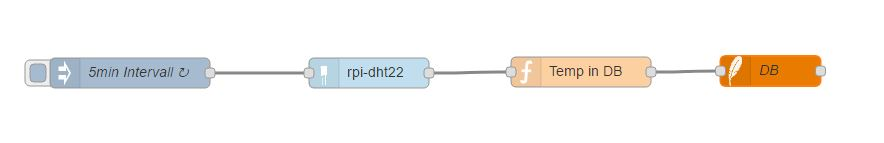
\includegraphics[scale=0.7]{images/tempIntoDB}
	\caption{Beispiel: Temperatur/ Luftfeuchtigkeit in Datenbank}
	\label{flow:tempDB}
\end{figure}
\begin{lstlisting}[label=list:tempIntoDB, caption={Neuer Eintrag in Tabelle DHT}]
var date = Date.now();
var newMsg = {
	"topic": "INSERT INTO DHT VALUES(NULL,"+msg.payload+","+msg.humidity+ ", '"+msg.sensorid+"', "+date+")"
}
return newMsg;
\end{lstlisting}


\subsection{Flows Node-Red}
Damit die gespeicherten Daten zu den verschiedenen Sensoren auch für andere Anwendungen bereitgestellt werden können, werden mithilfe des Node-Red-Webservers REST Servies angelegt. Diese können über \ac{HTTP} Anfragen angesprochen werden und liefern als Ergebnis Daten im \ac{JSON}-Format zurück. Dabei wird je nach angesprochenem Pfad ein bestimmtes Ergebnis zurückgeliefert. \\Anfragen müssen an den Raspberry Pi bzw. dessen Webserver-Schnittstelle gesendet werden. Dabei ist darauf zu achten, dass sich der Node-Red-Webserver unter der \ac{IP}-Adresse des Raspberry Pis und dem Port 1880 erreichen lässt. Als Beispiel könnte die Adresse folgendes Format haben: 192.168.0.100:1880. \\Damit nun ein entsprechender Service aufgerufen wird, muss noch eine Pfad an die \ac{URL} angehängt werden. In NOde-Red wurden folgende REST \ac{API} Schnittstellen entwickelt:
\begin{itemize}
	\item \textbf{/temp}: Diese Route liefert dem User den aktuellen, vom Temperatur- \& Luftfeuchtigkeitssensor gemessenen Wert zurück. 
	\item \textbf{/tempInt}: Um sich den Temperaturverlauf innerhalb eines begrenzten Zeitraums sich anzeigen zu lassen, kann diese Route angesprochen werden. Dabei müssen ein Startdatum, sowie ein Enddatum jeweils im Format \enquote{dd.mm.yyyy} als Parameter der Anfrage mit übergeben werden.
	\item \textbf{/window}: Gibt den aktuellen Status zurück, ob das Fenster geöffnet oder geschlossen ist.
	\item \textbf{/motion}: Liefert als Ergebnis eine ID, einen Zeitstempel zurück, um dem Anwender mitzuteilen zu welchem Zeitpunkt erkannt wurde.
	\item \textbf{/picture}: Dieser Service benötigt als Parameter eine ID, die über den Pfad \enquote{/motion} ermittelt werden kann. Durch diese ID kann dann der Pfad zum entsprechenden Bild geladen werden und als Antwort wird das Bild dem Anwender angezeigt.
	\item \textbf{/mqgas}: Die aktuellen Gas Werte können über den Services herausgefunden werden.
	\item \textbf{/gasInt}: Gleiches Prinzip, wie bei der Route \enquote{/tempInt}. Dem Request werden zwei Parameter (Startdatum, Enddatum) übergeben und die Gaswerte zurückgeliefert, die im angegebenen Zeitraum erfasst werden.
\end{itemize}

\autoref{flow:TempInt} stellt beispielhaft den Node-Red-Flow zum Abfragen des Temperatur- und Luftfeuchtigkeitsverlauf dar. Der Service wird angesprochen, wenn folgender Pfad adressiert wird: /tempInt?from=10.05.2017\&to=22.05.2017. Mit dieser Anfrage werden alle gespeicherten Werte als Antwort zurückgeliefert, die im entsprechenden Intervall liegen. wie der Node-Red-Flow zur entsprechenden Route 

\begin{figure}[h]
	\centering
	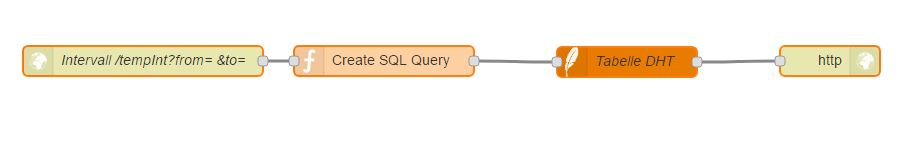
\includegraphics[scale=0.7]{images/tempIntFlow}
	\caption{Beispiel: Temperatur Intervall abfragen}
	\label{flow:TempInt}
\end{figure}
Der erste Node wird dazu benötigt, um eine HTTP Request anzunehmen. Dabei ist die Route zu definieren, unter der der Service erreichbar sein soll. In diese Fall ist dies \enquote{/tempInt}. Die übergebenen Parameter werden erst in Funktions-Knoten betrachtet, d. h. die eingehenden Parameter wurden über ein JSON-Objekt an den nachfolgenden Knoten übergeben. 
\\\autoref{list:tempInt} ist der Quellcode des Funktionsknotens. In Zeile 3 wird geprüft, ob beide Parameter gesetzt sind. Falls dies nicht der Fall ist sollen die letzten 20 Einträge aus der Datenbank geladen werden (siehe Zeile 24 \autoref{list:tempInt}). Dieser Schritt ist notwendig, da der nachfolgende Knoten auf die Datenbank zugreift. Liegt keine Abfrage vor, so wird ein Fehler zurückgeworfen und der Flow wird unterbrochen. 
\\Falls beide Parameter gesetzt wurden, müssen JavaScritp Zeitstempel generiert werden, da nur solche in der Datenbanktabelle DHT gespeichert sind. Hierfür werden in Zeile 10f die beiden Strings in Arrays unterteilt, sodass das Jahr, der Monat und die Tage separiert sind. Anschließend kann mithilfe des Date Objektes ein Zeitstempel generiert werden. Dabei ist darauf zu achten, dass JavaScript in den Monaten bei \enquote{0} zu zählen beginnt und somit der Monat um eins reduziert werden muss. \\Der timestampTo wird außerdem noch mit 23 Studen, 59 Minuten und 59 Sekunden erzeugt, damit ein einzelner Tag auch respektiert werden kann. \\Sobald beide Zeitstempel vorliegen wird die \ac{SQL} Abfrage generiert und in der Variable \enquote{selectString} gespeichert. \\Zum Schluss muss die Abfrage in einem JavaScript Objekt als Key-Value übergeben werden. Die Datenbankabfragen muss dabei immer unter dem Key \enquote{topic} abgelegt sein.  
\begin{lstlisting}[label=list:tempInt, caption={Funktion Node-Red tempInt}]
var selectString;

if(msg.req.query.from && msg.req.query.to){
	var fromDate = msg.req.query.from;
	var toDate = msg.req.query.to;
	
	/*convert date into timestamp
	first divide date string into day, month, year 
	then create new Date to get an timestamp*/
	var fDate = fromDate.split("."); 
	var tDate = toDate.split(".");
	
	/*create timestamp; month-1 because Jan = 0, Feb = 1 etc.
	date requires the order: year, month, day, hours, minutes, seconds */
	var timestampFrom = new Date(fDate[2], fDate[1]-1, fDate[0]).getTime();
	//to respect the whole day set hours, minutes, and seconds
	var timestampTo = new Date(tDate[2],tDate[1]-1, tDate[0], 23, 59, 59).getTime();
	
	var select = "Select * FROM DHT WHERE timestamp >= "; 
	var and = " AND timestamp <=";
	selectString =select + timestampFrom + and + timestampTo;
}
else {
	selectString = "Select * FROM DHT ORDER BY ID DESC LIMIT 20";
}

//create Message object for db access
var newMsg = {};
newMsg.topic = String(selectString);
return newMsg;
\end{lstlisting}

Nachdem die Abfrage im entsprechenden Objekt vorliegt kann der Datenbank Knoten die Anfrage verarbeiten und die ermittelten Ergebnisse werden an die \ac{HTTP} Node gesendet.
\\\autoref{list:temp}  zeigt das \ac{JSON}, das von Webserver als Antwort zurückgeliefert wird. Dieses hat durchgehend die gleiche Struktur und kann somit nach den Key-Value-Prinzip ausgelesen werden. Enthält eine Antwort mehrere Einträge, wird ein Array mit mehreren Objekten zurückgeliefert.
\begin{lstlisting}[label=list:temp, caption={JSON Response /temp}]
{
	"temp": "24.60",
	"humidity": "46.60",
	"sensorid": "dht22",
	"date": 1495920298490
}
\end{lstlisting}


\section{Grafische Benutzeroberfläche} %Louisa
Als grafische Benutzerschnittstelle für das in dieser Arbeit erläuterte System wird eine ortsunabhängige Lösung entwickelt (F-10.2). Um eine Ortsunabhängigkeit gewährleisten zu können, bietet es sich an ein mobiles Endgerät zu entwickeln. Es wurde  entschieden als Benutzerschnittstelle eine Android App zu nutzen, aus dem Grund, dass Android den höchsten Endkundenabsatz besitzt \cite{statista:marktanteileandroid} und dadurch eine größere Masse erreicht werden kann.
\subsection{Rule Engine}
Die Rule Engine wird nach den Anforderungen aus Kapitel \ref{sec:Anforderungen} entwickelt. Demnach muss die Rule Engine dem Nutzer ermöglichen dynamisch Regeln hinzufügen zu können oder wieder zu löschen (F-30.1). Grenzwerte oder Wertebereiche kann der Nutzer für die erfassten Datentypen (F-10) selbst bestimmen (F-30.2). Des Weiteren soll die Rule Engine zeitliche Aspekte in den Regeldefinitionen einbinden können. Der Nutzer kann demnach zeitliche Intervalle festlegen, in denen ein Wert oder Wertebereich gehalten werden soll. Die Definition von Datenabhängikeiten kann von der Rule Engine verarbeitet werden, um optimalere Aktionen auslösen zu können (F-30.5).\\
Es werden mögliche Rule Engines recherchiert, die die gestellten Anforderungen erfüllen. Dabei wurden nur Rule Engines betrachtet, die in Android genutzt werden können, sowie welche mit regelmäßigen Releases. Aus der Recherche haben sich folgende Rule Engine Bibliotheken ergeben:
\begin{itemize}                                                                                                                                                                                                                                                                                                                                                                                              
	\item Easy Rules \cite{github:easyrules}
	\item OpenRules \cite{openrules}
	\item RuleBook \cite{github:rulebook}
\end{itemize}
Diese Rule Engines bieten gute Möglichkeiten Regeln zu erstellen und diese zu überprüfen. Der entscheidene gemeinsame Nachteil dieser Rule Engines ist die Implementierung der Regeln. Durch die Recherche konnte keine Engine gefunden werden, die eine dynamische Erstellung von neuen Regeln über die Oberfläche ermöglichen. Die Definition neuer Regeln durch den Nutzer ohne den Quellcode zu verändern ist jedoch eine essentielle Anforderung. Aus diesem Grund wurde sich dafür entschieden, eine Rule Engine selbst zu implementieren.\\
Bei der Implementierung der Rule Engine wurden die Ergebnisse der Recherche miteinbezogen. Vor allem an die Struktur der Regeln zu ihren Wenn- und Dann-Teilen der Regel Engine RuleBook wurde bei der Implementierung betrachtet.


- Warum keine RuleEngine Bibliothek nutzen?
-mögliche Rule Engines: es wurden nur RuleEngines betrachtet, die in Android genutzt werden können
- Easy Rules
- OpenRules
- Dredd
- RuleBook
-Vorteile:  
- Nachteile bzw. Vorteile von diesen Engines
- Warum keine bekannt Rule Sprache nutzen um Regeln zu definieren? - RuleML

\subsection{Daten Anzeige}